\documentclass[e4_tp2_main.tex]{subfiles}
\begin{document}
\newgeometry{top=2.5cm, bottom=2.0cm, left=2.25cm, right=2.25cm}

\section{Convertidor Boost para Lámpara LED de potencia}

\subsection*{LED's de Potencia: Efecto de la temperatura - Realimentación}
De la hoja de datos de OSRAM para el LUW-W5AP, se da la curva de $\Delta V(T)=V_F-V_F(25^{\circ})$, para la corriente $I_F$ máxima de 1400mA. La misma tiene pendiente negativa, es decir, que a mayor temperatura, la tensión en directa sobre el LED disminuye.

\begin{figure}[H]
\centering
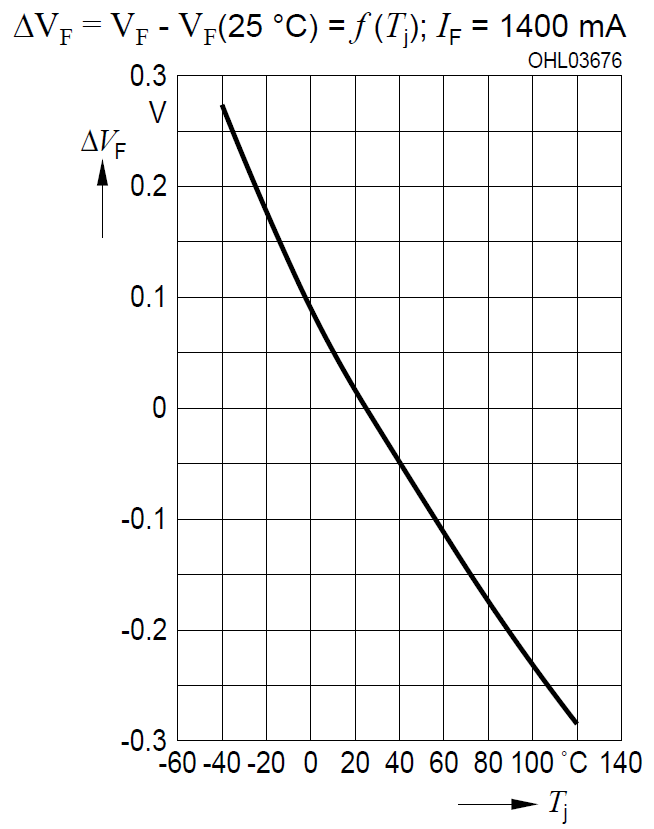
\includegraphics[width=0.3\linewidth]{Imagenes/Punto2/efectoT.png}
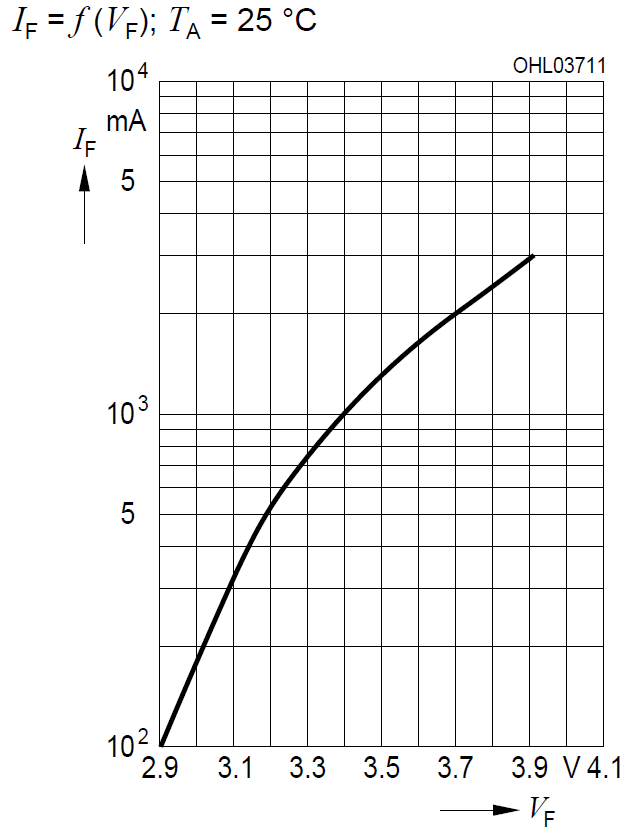
\includegraphics[width=0.29\linewidth]{Imagenes/Punto2/IF-VF.png}
\caption{Efecto de la temperatura en la $V_{LED}$ - Curva de $I_F(V_F)$}
\end{figure}

Al trabajar con LED's de potencia, es conveniente realimentar la corriente en lugar de la tensión. Esto se debe a que si se produce una perturbación en la carga (es decir, para el caso de la simulación cortocircuitar dos LED's), si se está regulando tensión, caerá más tensión sobre los LED's restantes, por lo que la corriente aumentará, de acuerdo a la curva de $I_F(V_F)$ provista en la hoja de datos.

\end{document}